% arara: xelatex: {shell: true}
% arara: biber
% arara: xelatex: {shell: true}
% arara: xelatex: {shell: true}
\documentclass[letterpaper,10pt]{article}
\usepackage[margin=1in]{geometry}
\usepackage{hyperref}
\usepackage{graphicx}
\usepackage[justification=centering,font=small,labelfont=bf]{caption}
\usepackage{fancyhdr}
\usepackage{fontspec}
\usepackage{relsize}
\setmonofont{Inconsolata}[Scale=MatchLowercase]
\defaultfontfeatures{Ligatures=TeX}
\usepackage{xeCJK}
\usepackage{minted}
\usepackage{xcolor}
\definecolor{dsscawpurp}{HTML}{b079b0}
\definecolor{dsscawpurpcap}{HTML}{6c286c}
\usepackage[font={color=dsscawpurpcap},labelfont={sc}]{caption}
\usepackage[backend=biber,
date=iso,
seconds=true,
style=numeric,
bibencoding=utf8,
]{biblatex}

\addbibresource{\jobname.bib}
\usemintedstyle{colorful}
\newenvironment{denseitemize}{
  \begin{itemize}
      \setlength{\itemsep}{0pt}
}{
  \end{itemize}
}
\newcommand\CC{C\nolinebreak\hspace{-.05em}\raisebox{.4ex}{\relsize{-3}{\textbf{+}}}\nolinebreak\hspace{-.10em}\raisebox{.4ex}{\relsize{-3}{\textbf{+}}}\hspace{.2em}}

\pagestyle{fancy}
\rhead{
  
\includegraphics[height=\fontcharht\font`\D,keepaspectratio=true]{../dsscaw-hdr.pdf}
  \textcolor{dsscawpurp}{DSSCAW Technical Report \#002}
}

\title{µnandfs:\\
A NAND Blobstore for Memory-Starved Platforms\thanks{
 \href{https://www.dsscaw.com/}{Dirty South Supercomputing} on behalf
 of \href{https://www.vakaros.com/}{Vakaros} of Atlanta, GA.
}\\
}
\author{Nick Black, Consulting Scientist\\
\texttt{nickblack@linux.com}
}

%%%%%%%%%%%%%%%%%%%%%%%%%%%%%%%%%%%%%%%%%%%%%%%%%%%%%%%%%%%%%%%%%%%%%%%%
\begin{document}
%%%%%%%%%%%%%%%%%%%%%%%%%%%%%%%%%%%%%%%%%%%%%%%%%%%%%%%%%%%%%%%%%%%%%%%%
\maketitle
\thispagestyle{fancy}
\date{}
\begin{abstract}
I was tasked with designing and implementing a persistent associative array
mapping names to arbitrary data---i.e. a single-directory filesystem, often
called a \textit{blobstore}---using the Nordic Semiconductor nRF52840 SoC and
two Winbond W25N01GV gigabit SLC NAND chips. The contract also required
necessary QSPI drivers. The requirements permitted 4KB of RAM, allowed no use
of other persistent storage, and mandated a fully asynchronous API running on
``bare metal'' (no OS, realtime or otherwise). I detail my resulting
deliverable, µnandfs, and demonstrate its generally performant and robust
fulfillment of these specs. I also describe its pathological worst case
behaviors.
\end{abstract}
%%%%%%%%%%%%%%%%%%%%%%%%%%%%%%%%%%%%%%%%%%%%%%%%%%%%%%%%%%%%%%%%%%%%%%%%
\section{Introduction}
The client's initial request was simply ``a filesystem on the nRF52840 using
two W25N01GV NANDs, plus any necessary drivers, plus an entirely asynchronous
\CC API, in as little RAM as possible''. Refinement of these requirements
determined that:
\begin{denseitemize}
\item Most files would be on the order of 1KB, with a few files
       on the order of tens of megabytes. These larger files would grow
       over time, via substantial (page-sized) appends.
\item It was not thought necessary to have directories, nor links (either hard
       or symbolic), but it must be possible to remove files, reclaiming both
       their space and name.
\item It must be possible to have multiple files open at once, but it is not
       necessary that a single file support multiple open handles. Writing
       to a file need not be visible to an existing reader.
\item No more than 4KB of RAM was to be consumed, and ideally not more than 2KB
       would be persistently consumed. Callers could be required to supply
       an additional 2KB for the duration of their operation.
\item Wear-leveling must be as close to uniform as possible. Ideally, no block
       would be erased two times more than any other block. Robustness in
       general is at a premium.
\end{denseitemize}

The nRF52840\parencite{nrf52840} SoC pairs an ARM Cortex-M4F with 1MB of
NOR flash and 256KB of RAM, along with a wealth of interconnection
capabilities. This storage is shared with the ``S140
SoftDevice''\parencite{s140}, a closed-source BlueTooth stack, which consumes
slightly more than 100KB of RAM and significant flash.
Two Winbond W25N01GV\parencite{winbond}
128MB NANDs, each capable of QSPI at up to 104MHz, were added to the PCB.
One QSPI and three SPI masters are available, each clocked at 32MHz (ignoring
overhead, 32MHz QSPI moves an ideal 16MB/s, SPI a respectable 4MB/s). Nordic's nRF5 SDK\parencite{nrf52sdk}
version 15.3.0 was linked into our binary, and the DUT was probed via 10-pin
J-Link\parencite{segger} connection from an nRF52-DK\parencite{nrf52dk}.

\section{Details of NAND flash}

NAND flash---typically packaged as a collection of chips, and often managed via
an on-board controller---makes up the majority of modern solid state drives,
flash drives, and memory cards. It is cheaper and denser than NOR flash,
faster than spinning disk, \textit{much} faster than EEPROMs, but typically
less reliable than any of the three. There are severe constraints on how it can be
used: a chip of NAND flash is divided into some number of \textit{blocks}, which are
themselves divided into \textit{pages}. Erasing a block changes all bits within to
1s\footnote{Nothing about the NAND memory cell itself---floating-gate MOSFETs
connected in series---requires large-scale operations. Larger blocks mean
faster operations (per bit), cheaper chips, and less power draw\ldots plus
amplified errors, and reduced flexibility.}. Data can be written a page at a
time within a block, but usually only in ascending page order---out-of-order
page programming can upset data in adjacent wordlines (a ``program
interference``\parencite{interference}). Data can be read a page at a time from
anywhere within the block, but reading a page too many times can upset data in
an adjacent page (a ``read disturb''\parencite{readdisturb}). SLC NAND flash stores one bit per cell,
and blocks can be erased on the order of $10^5$ times. MLC and TLC variants
encode more bits per cell, and can be reliably erased far fewer times (they
also tend to be slower, and to require more ECC bits per data bit). As a block
wears out, programming time will decrease, while erase latency
increases\parencite{needtoknow}. Finally, it is common for MLC and TLC NAND to
exhibit ``fast pages'' and ``slow pages'', but this arises from the
distribution of bits within a multilevel cell to different pages, and thus does
not affect SLC NAND\parencite{anomalies} such as our Winbond.

\subsection{Details of the Winbond W25N01GV}
The W25N01GVxxIG/IT\footnote{The ``xx'' is a package code, one of ZE (WSON), SF (SOIC),
or TB/TC (TFBGA). IG/IT differentiates between devices which reset into ``continuous mode''
or ``buffered mode''. We always use the (default) buffered mode on our IGs.} is
organized as $2^{10}$ blocks of $2^6$ 2KB pages each ($2^{17}$ bytes per block), for
a total of $2^{16}$ pages and $2^{27}$ data bytes (128MB). Blocks must be
erased before their pages can be programmed with 0s, and pages must be
programmed in ascending order. A page may be read from any block at any time.
In addition to the 2KB of data, each page has a 64 byte ``Spare Area'',
primarily used for hardware-managed ECC\footnote{Those who long to live
dangerously can disable hardware ECC. We don't.}, but offering 16 ECC-protected bytes
(in 4 discontiguous 4-byte chunks) for our use. A bad block mapper (BBM) of 20
LUTs is at our disposal, providing transparent remapping of block addresses.
Finally, there are 10 ``One-Time Program'' pages, which can be written to only
once.

Block erasure operations can fail, setting the FAIL-E bit; likewise page
programming and FAIL-P. Both of these bits are reset when the next operation
is started. Page read operations that fail their ECC check result in one or
more ECC error bits being set. These error bits remain high until the chip is
reset. Most operations set the BUSY bit, and only when this bit goes low is it
safe to consider an operation completed.

\subsection{Interactions with the nRF52840}
The Winbond's command set bears no resemblance to the ONFI
standard\parencite{onfi}, so there's no need to learn the latter. Unfortunately,
it also differs wildly from that supported by the nRF52840's QSPI
interface. Extensive use of the {\texttt{CINSTR}} ``custom instruction''
facility was needed, but eventually full-speed communication was had over
QSPI with the two NANDs. Alas, the Nordic unit can only deal with pages of
either 256 or 512 bytes. Using the maximum 512 byte setting, the last 512 bytes
written anywhere in the page would be returned for subsequent reads from the
page of any length. Eventually, it was confirmed with Nordic support that their
QSPI controller simply can't drive a 2KB page for more than 25\% of its
capacity. A bit-banging approach, were it even possible to do robustly,
would consume far too many CPU cycles (remember, all interfaces were to be
asynchronous). Faced with either a 75\% reduction in speed or a 75\% reduction
in capacity, the clients chose to retain capacity, and we moved to the SPI interfaces.
Note that hanging both chips off the QSPI interface meant that only one would
be used at a time (aside from a mirrored configuration employing
``superblocks''\parencite{superblocks}), but placing the two on distinct SPI
interfaces allows for parallelism. Full, concurrent utilization of both SPIs would represent
50\% of the original QSPI throughput.

\section{Blobstore API}
I had some ideas regarding the internal design, taking inspiration from
classic work on log-structured filesystems\parencite{sprite}, particularly
as implemented in NAND-focused projects such as F2FS\parencite{f2fs},
JFFS2\parencite{jffs}, and YAFFS\parencite{yaffs}. At the same time, I wanted
a simpler scheme, one implementable in 2KB of RAM, by one engineer, in four
weeks of part-time work. These ideas informed the proposed API, which happily
ended up pretty well-suited to the final implementation.

\begin{listing}[ht]
\caption{Public API ({\texttt{NANDDev}} defines CS pin and SPI device)}
\begin{minted}{C++}
constexpr size_t BLOB_NAME_MAXLEN = 58; // Including mandatory NUL byte!
constexpr auto NAND_PAGE_DATABYTES = 2048u;
constexpr auto NAND_PAGE_SPAREBYTES = 64u;
constexpr auto NAND_PAGE_SIZE = NAND_PAGE_DATABYTES + NAND_PAGE_SPAREBYTES;

using blob_t = uint64_t;
using NANDPage = std::array<uint8_t, NAND_PAGE_SIZE>;
using Handler = void(*)(void *, int);
using FSCallback = void(*)(void*, blob_t, size_t);
using FSCtx = std::pair<FSCallback, void*>;

class VK_FS {
 static int Format(Handler fxn, void* vctx, NANDDev* nand);
 template<class It> int Init(Handler fxn, void* vctx, It begin, It end, bool mirror);
 int Fsck(Handler fxn, void* vctx, bool checkdata);
 // flags include BLOB_CREAT, BLOB_EXCL, and BLOB_KILL
 blob_t OpenBlob(const std::string& name, unsigned flags, const FSCtx& ctx);
 blob_t ExtendBlob(blob_t blob, const void* buf, size_t len, const FSCtx& ctx, NANDPage& scratch);
 blob_t ReadBlob(blob_t blob, void* buf, size_t len, unsigned offset, const FSCtx& ctx, NANDPage& scratch);
 blob_t Bloblen(blob_t blob, const FSCtx& ctx, NANDPage& scratch);
 blob_t CloseBlob(blob_t blob, const FSCtx& ctx);
 blob_t ReplaceNamedBlob(const std::string& name, const void* buf, size_t len, const FSCtx& ctx);
 blob_t RemoveNamedBlob(const std::string& name, const void* buf, size_t len, const FSCtx& ctx);
 blob_t ListBlobs(blob_t blob, const FSCtx& ctx, NANDPage& scratch);
 blob_t Sync(const FSCtx& ctx);
 int Reset();
}
\end{minted}
\end{listing}

A {\texttt{NANDDev}} is a small structure, often {\texttt{constexpr}}, tying
together a SPI master identifier and a Chip Select line (numerous slaves can be
connected to a single SPI master, and selected via this line). The same {\texttt{NANDDev}}
must not be provided to two {\texttt{VK\_FS}} objects. To {\texttt{Format}} a
\texttt{NANDDev} is simply to erase all of its blocks, restoring all bits to their default
1. {\texttt{Init}} is handed one or more {\texttt{NANDDev}}s, and the boolean
{\texttt{mirror}} (if false, the NANDs are put in linear combination). All
specified devices must be freshly formatted, or they must make up an existing
filesystem (by virtue of having previously been fed together to
{\texttt{Init}})\footnote{In most mirrors, we'd want to be able to add a
  replacement device, but that won't be happening with our PCB in the field.}.
If {\texttt{Init}} is able to recognize the devices, it calls back with
success, and the object can be used until a call to {\texttt{Reset}}.

Functions will generally return {\texttt{BLOBD\_EINPROGRESS}}, and call back
asynchronously with the true handle. Callers must be prepared for an immediate
return, however, in which case no callback will be invoked. The proper idiom
is thus typically to invoke the function, check if the result is
{\texttt{BLOBD\_EINPROGRESS}}, and if not, directly invoke the callback
from the original callsite. The primary handle provided to callers is the
{\texttt{blob\_t}}\footnote{We encode all handle state in the \texttt{blob\_t},
  held by the client. ``File descriptors'' imply indices into space
  proportional to the number of open handles, a luxury we're not afforded.}.
This 64-bit value is opaque to callers except through the following two
functions:

\begin{listing}[ht]
\caption{Functionality for inspecting {\texttt{blob\_t}}}
\begin{minted}{C++}
// Returns true iff the blob_t is an error code
static inline bool BlobErrorP(blob_t code) {
  return code & 0x3ul;
}

// Errors can be any arbitrary distinct blob_t with a 1 in the LSB. Each of
// these is all 1s, except for one low bit (for differentiation).
constexpr blob_t BLOBD_EINPROGRESS = ~(0x1u << 22); // request not yet complete
constexpr blob_t BLOBD_EIO = ~(0x1u << 23); // error talking to device
constexpr blob_t BLOBD_ENOSPC = ~(0x1u << 24); // no room to write
constexpr blob_t BLOBD_ENOENT = ~(0x1u << 25); // no BLOB_CREAT, but blob did not exist
constexpr blob_t BLOBD_ENAMETOOLONG = ~(0x1u << 26); // no NUL in 58 bytes of name
constexpr blob_t BLOBD_EINVAL = ~(0x1u << 27); // bad flags or invalid blobd or invalid read length
constexpr blob_t BLOBD_EEXIST = ~(0x1u << 28); // blob existed with BLOB_EXCL
constexpr blob_t BLOBD_INVALID = ~0ul; // generic error

static inline const char* BlobStrerror(blob_t res) {
  switch(res){
    case BLOBD_EINPROGRESS: return strerror(EINPROGRESS);
    case BLOBD_EIO: return strerror(EIO);
    case BLOBD_ENOSPC: return strerror(ENOSPC);
    case BLOBD_ENOENT: return strerror(ENOENT);
    case BLOBD_ENAMETOOLONG: return strerror(ENAMETOOLONG);
    case BLOBD_EINVAL: return strerror(EINVAL);
    case BLOBD_EEXIST: return strerror(EEXIST);
    case BLOBD_INVALID: [[fallthrough]];
    default:
      if(BlobErrorP(res)){
        return "Unknown unandfs error";
      }else{
        return strerror(0);
      }
  }
}
\end{minted}
\end{listing}

{\texttt{OpenBlob}} searches for the specified name, and then functions according
to the provided flags. If {\texttt{BLOB\_CREAT}} is provided, the blob will be
created if it does not yet exist (without \texttt{BLOB\_CREAT}, {\texttt{BLOBD\_ENOENT}} would
be returned). If {\texttt{BLOB\_EXCL}} is provided (providing {\texttt{BLOB\_EXCL}}
without {\texttt{BLOB\_CREAT}} results in {\texttt{BLOBD\_EINVAL}}), the
blob \textit{must not} exist, or \texttt{BLOBD\_EEXIST} will be returned. If
\texttt{BLOB\_KILL} is provided (providing \texttt{BLOB\_KILL} with \texttt{BLOB\_CREAT}
results in \texttt{BLOBD\_EINVAL}), the blob will be removed if it exists (otherwise,
\texttt{BLOBD\_ENOENT} is returned). All other errors can also occur with these
functions. The handle can now be used in calls to \texttt{ReadBlob}, \texttt{ExtendBlob},
\texttt{Bloblen}, and \texttt{CloseBlob}. Behavior is undefined if the blob
is modified through another handle or function. Failure to call \texttt{CloseBlob}
does \textit{not} cause a resource leak, but timely use of \texttt{CloseBlob}
can result in fewer wasted NAND pages.

\texttt{ExtendBlob} adds up to a page worth of data to the blob. The callback
specifies a new handle which should be used for further extensions (extending
again on the same blob will replace the extended data). No matter the extension's
length, a full page will be consumed for the data, plus an inode ($\frac{1}{32}$
of a page) to describe the data page; it is thus desirable for callers to
buffer a full page worth of output. A blob can grow as large as $2^{24}-1$
bytes (16MB; this is the sum of actual data, not consumed pages). Note that
other handles will not be updated; it is not possible for a reader to notice
the new data save by calling \texttt{OpenBlob} anew. The amount written is
returned as the third argument to the callback.

\texttt{ReadBlob} allows up to a page worth of data to be read from the blob,
at the specified offset. If the requested amount of data is not available, a
short read will be returned as the third argument to the callback. \texttt{Bloblen}
gets the length of the blob through this handle (again, concurrent extensions
will not be visible). \texttt{CloseBlob} hints that no more extensions will
be performed through this handle.

\texttt{RemoveNamedBlob} and \texttt{ReplaceNamedBlob} skip the name lookup
procedure, forcefully seizing the name and either marking it dead, or
initializing it with up to one page of data. Extending a handle which has been
\texttt{Remove}d or \texttt{Replace}d leads to frightful shenanigans (typically,
the old blob will ``return from the grave'').

\texttt{ListBlobs} ought first be called with \texttt{BLOBD\_INVALID}. It will
populate \texttt{scratch} with between 1 and 31 blob names and lengths, and
return a nonce \texttt{blob\_t}. This can be used in a subsequent call, which
will return a new nonce, and a new set of blob names and lengths. Eventually,
\texttt{BLOBD\_ENOENT} will be returned, and all blobs will have been
enumerated. I have not bothered to include the functions for extracting these
data.

\texttt{Sync} ought be called prior to \texttt{Reset} or process exit. Any
metadata not yet written to NAND will be flushed. Calling \texttt{Sync} can
waste up to 62 pages, so do it only when necessary. Failure to call \texttt{Sync}
can currently result in up to 61 pages being lost. \texttt{Fsck} can be used to
perform an intensive validation of the filesystem, requiring a read of every
metadata page ($\frac{1}{32}$ of the pages). If \texttt{checkdata} is true, \texttt{Fsck}
will read every page of the NAND, looking for ECC errors. In the absence of
any other load, this requires roughly 42s per NAND.

All of these functions can involve some asynchronous I/O. In the best case,
necessary information is readily available in the active metadata, and the
return is immediate. Extending a blob can result in up to two pages being
written out in the active block, and a full block copy if space needed to be
found in a used block (but will usually result in one page being written).
In the worst case, where the named blob does not exist on a full NAND, a name
lookup requires reading every metadata page. Creating (or removing) a file
usually leads to no I/O, but in the worst case leads to a page being written
out followed by a block copy. Reading a blob requires traversing some number of
metadata pages; in the worst case, where a blob has grown fat off partial
writes, this could again require reading every metadata page (see
Section \ref{futurework} for plans on improving this linear behavior on reads).

\texttt{BLOB\_NAME\_MAXLEN} is derived from filesystem internals, as we shall
now see.

\section{Filesystem design}

I knew I wanted to provide at least a few dozen bytes' worth of name per blob.
I knew 16 bits of blob length were too little, and 32 bits too much.
I considered metadata compression, and said ``no'' to madness.

I knew I wanted to march purely forward writing within a chip---i.e., in
addition to the mandatory in-order programming of pages, I hoped to erase
blocks in order, with no special meaning for any given block. Any such scheme
is guaranteed perfectly uniform wear leveling, and should require minimal state
(I knew that any frequently-changing state couldn't be persisted without either
redundancy or special-purpose blocks). I considered bundling metadata with
data. Such a scheme would be very flexible; I could write the metadata length
and true length into the Spare Area, grow the data up from the bottom and the
metadata down from the top, and have type-tagged metadata tuned to the particular
blob. I could even pack multiple small blobs into a single page. Unless I
wanted to buffer data across calls there was no way for a caller to know how
much data to optimally pass with variable-length, in-page metadata. Buffering
would require RAM linear with the number of incomplete writes, though, so it
was out. Metadata and data would live on different pages, and I'd burn my
allotted 2KB building up the next metadata page in memory.

A problem presented itself, however: how would I determine state on
initialization? As noted above, if I persisted my state
to a known location, those locations would see significant wear. Under the
mixed pages plan, every page had identifiable metadata, and that metadata could
carry a decreasing nonce. Find the discontinuity in nonces, and you've found
your active page (more on this momentarily). By placing metadata pages at the
32nd and 64th page of each block, nonces can be recorded in these pages only, and
the same $\mathcal{O}(\log{}n)$ algorithm performed (on $\frac{1}{32}$ as many pages). I call these
32-page regions \textit{zones}. This yielded up a natural 64-byte fixed inode
size for each of the 31 previous pages, plus 64 bytes for zone metadata. Three
bytes were dedicated to ``blob length through this inode'', two bytes to
``previous data page'' (the data page governed by an inode can be derived in
$\mathcal{O}(1)$, as can the inode corresponding to a data
page), and one byte to a status bitfield. The remaining 58 bytes became
\texttt{BLOB\_NAME\_MAXLEN}\footnote{Metadata placed flexibly, only when
  appropriate for recent I/O, could be more efficient than periodic metadata
  with a fixed inode size (fewer pages used for metadata, fewer pages needing
  reading to describe a given file). Metadata and arbitrary data pages could be
  differentiated via a single bit in the Spare Area. Finding the metadata page
  describing a given data page becomes $\mathcal{O}(\log{}n)$ as opposed to
  $\mathcal{O}(1)$.}.

We define a few useful functions before proceeding:

\begin{listing}[ht]
\caption{Functionality for navigating data and metadata pages, all $\mathcal{O}(1)$}
\begin{minted}{C++}
constexpr size_t INODE_SIZE = 64;
static_assert(NAND_PAGE_DATABYTES % INODE_SIZE == 0);
constexpr auto PAGES_PER_ZONE = NAND_PAGE_DATABYTES / INODE_SIZE;
static_assert(PAGES_PER_ZONE > 1 && ((PAGES_PER_ZONE & (PAGES_PER_ZONE - 1)) == 0);
constexpr auto DATA_PAGES_PER_ZONE = PAGES_PER_ZONE - 1;
constexpr auto LAST_METADATA_PAGE = NAND_BLOCK_COUNT - 1;

static inline unsigned // Given a raw page, return its associated metadata page and zidx
MetadataForPage(unsigned pidx, unsigned* zidx) {
  if(zidx){
    *zidx = pidx % PAGES_PER_ZONE;
  }
  return pidx | DATA_PAGES_PER_ZONE;
}

static inline unsigned // Given a metadata page and inode number, return described page
PageMetadataOwns(unsigned pidx, unsigned zidx) {
  return (pidx & ~DATA_PAGES_PER_ZONE) + zidx;
}

static inline unsigned // Return metadata page of next zone
NextMetadataPage(unsigned pidx) {
  pidx = MetadataForPage(pidx, nullptr);
  return (pidx == LAST_METADATA_PAGE) ? DATA_PAGES_PER_ZONE : pidx + PAGES_PER_ZONE;
}

static inline unsigned // Return metatdata page of previous zone
PrevMetadataPage(unsigned pidx) {
  pidx = MetadataForPage(pidx, nullptr);
  return (pidx == DATA_PAGES_PER_ZONE) ? LAST_METADATA_PAGE : pidx - PAGES_PER_ZONE;
}

static inline unsigned // Return epoch corresponding to nonce
EpochForNonce(uin32_t nonce) {
  return ((uint64_t)0xffffffffull - nonce + NAND_BLOCK_COUNT - 1) / NAND_BLOCK_COUNT;
}
\end{minted}
\end{listing}

\begin{minipage}{\textwidth}
\begin{center}
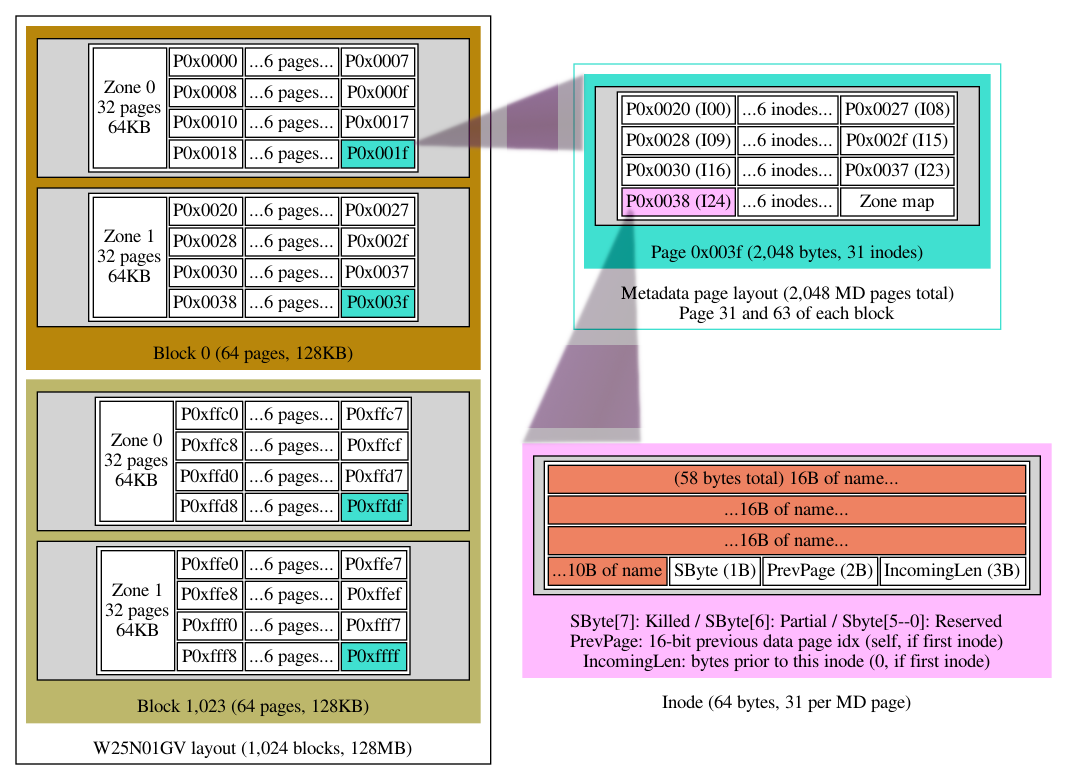
\includegraphics[width=.8\linewidth]{combined.png}
\captionof{figure}{Structure of chip, block, metadata page, and inode}
\end{center}
\end{minipage}

\subsection{Phased algorithm for block movement} \label{shuffle}
That's all well and good, but what becomes of our ineluctable march when we
wrap around to the front of the NAND, and can't blow away live data? We
sacrifice one block worth of capacity, designating it the \textit{victim
  block}. On first initialization, this is the last block. We keep a counter,
initialized to 0 and increased by 1 each time we erase the first block,
designating it the \textit{epoch}. Note that we can derive the epoch from a
nonce in $\mathcal{O}(1)$, and that epochs partition the nonce space.

Whenever our current block becomes the victim block (this won't happen until the
last block, but it will happen every other zone afterwards), designate the subsequent
block to be the \textit{Dunkirk block}. Load the Dunkirk block's first zone's
metadata page as the working page. Beginning with the first inode, check to
see if it's dead. If so, it doesn't need rescuing; use its slot in the victim
to write the next data page. If it is live, copy it into the victim block to
fight another day. Copy pages in bursts when appropriate, and when the zone is
complete, write metadata to the victim block. Repeat this with the second zone.
Designate the Dunkirk block the victim block, and start over.

This maintains perfect wear leveling, and ought even perform reasonably well
when there are plenty of deletions. But what about outstanding handles to the
Dunkirk block? Their data just moved out from underneath them\footnote{We don't
guarantee other writers to be reflected in readers, but we can't very well
go shifting the world around \textit{ourselves}.}! Twenty bits in
each \texttt{blob\_t} are thus used to encode its origin epoch, i.e. the epoch
at the time of \texttt{OpenBlob}. If a \texttt{blob\_t} is handed to us with
our epoch, there's no way it's been moved. Otherwise, it has been moved zero or
more times; this can be computed in $\mathcal{O}(1)$, and applied to the incoming physical
location as an $\mathcal{O}(1)$ displacement modulo \texttt{NAND\_BLOCK\_COUNT}. This
method also effects perfect \textit{data scrubbing}\parencite{management},
the most effective solution for retention errors. In honor of minimalist
composer Stephen Reich, I refer to this movement of data as ``phase music''.

\subsection{Initialization algorithm} \label{callzones}
Knowing that freshly-formatted or otherwise erased blocks are all 1s, and
knowing that we write a decreasing nonce to each zone we write out, and knowing
that we write zones in order, lower to higher numbers, a valid µnandfs can take
one of three forms:
\begin{denseitemize}
\item \textit{More than two zones have a nonce of all 1s, these zones are
    contiguous, and they include the last zone. All other zones form a
    decreasing procession.} The µnandfs is freshly initialized, or was interrupted
    in its first epoch. The current zone is the first zone with an
    all-1s nonce.
\item \textit{Exactly one or two zones, within the same block, have a nonce of
    all 1s. All other zones form a decreasing procession.} The µnandfs was
  interrupted near the ends of its first epoch, or after erasing the current
  block.  The current zone is the first zone with an all-1s nonce.
\item \textit{All zones form a decreasing procession, save for a single discontinuity,
    when the nonce increases by the number of zones.} The µnandfs, in at least
    its second epoch, was interrupted before erasing the current block.
    The current zone is the zone with the greatest nonce.
\end{denseitemize}
If we're not concerned with verifying these properties in full (that's left to
the optional \texttt{Fsck}), we can recover the current zone in all three cases
with a single $\mathcal{O}(\log{}n)$ algorithm, one very much like binary search. First, note that if we
assume the remainder of the nonces to be in order, we can determine in $\mathcal{O}(1)$ 
whether a given zone is the current zone: if its nonce is greater than the
nonce of the previous zone, or if its nonce is all 1s and it is the first zone,
it can be considered the current zone (otherwise, if the previous nonce is not the
zone's nonce plus 1, and either nonce is anything but all 1s, there is
invalid metadata).

Read the nonces of the first, last, and (first + ((last - first) / 2)) zones.
If last is first's previous zone (as it will be on the first iteration),
determine if the first zone is current (as it will be on the first iteration).
Otherwise, read first's previous zone's nonce, and perform the same
decision. If not, get the middle zone's previous zone (which might be first),
and determine if the middle zone is current. If not, get the last zone's previous
zone (which might be mid), and determine if the last zone is current. If none
of the three were current, one of three cases is true:
\begin{denseitemize}
\item \textit{Middle nonce was less than first nonce and last nonce.} Set first zone
  equal to middle's successor, and last equal to last's predecessor, and loop.
\item \textit{Middle nonce was greater than first nonce and last nonce.} Set
  first equal to first's successor, and last equal to middle's predecessor, and
  loop.
\item \textit{Anything else.} Oh no look no, bad metadata, abandon ship.
\end{denseitemize}

\begin{minipage}{\textwidth}
\begin{center}
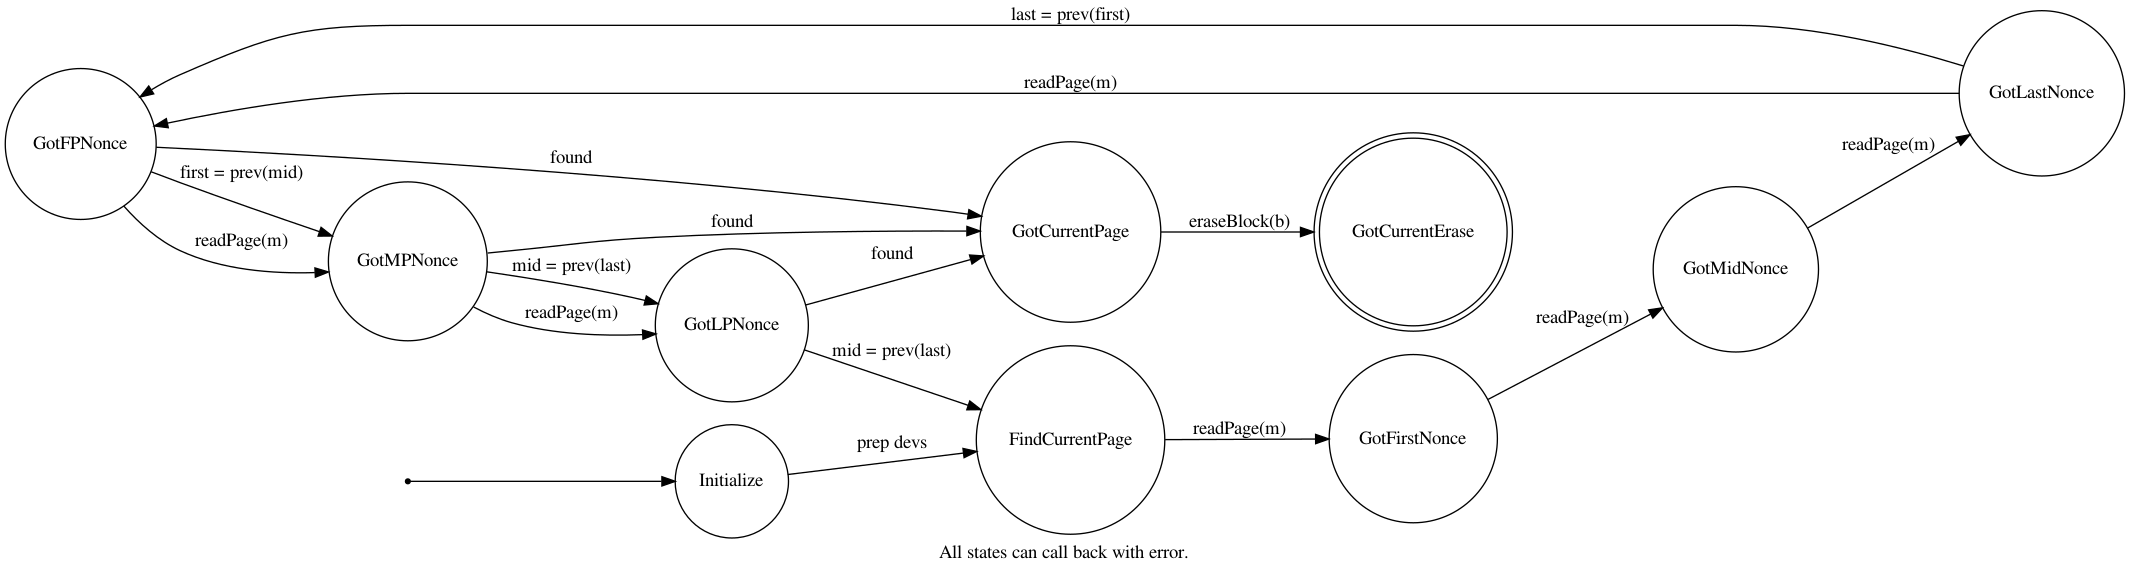
\includegraphics[width=1\linewidth]{Initialize.png}
\captionof{figure}{\texttt{Initialize} state machine}
\end{center}
\end{minipage}

In honor of Atlanta rappers the Ying-Yang Twins, I refer to this process as
``Calling all Zones\footnote{In truth, of course, we call only logarithmically
  many zones.}''.

\subsection{Name resolution and fast name operations}
The chip might have any number of instances of a particular name on it, with
pages in any order. Since we're always moving forwards through the chip, though,
we can order events. Start by searching through any active metadata, and then move
backwards through metadata pages until hitting an all 1s nonce, coming back to
the starting point, or finding an inode with the name. The most recent inode
of this epoch, if any exist, must be the most recent inode, and the lookup is
complete. If an inode is found which is not from this epoch, it is possible that
inodes ahead of us on the NAND have a newer, authoritative entry. Remember that
when shuffling pages from the Dunkirk block to the victim block, we must determine
whether they're live, which requires determining the authoritative end of the
blob. At that time, we write said end into the first two bytes of the Spare Area.
Since any inodes of a previous epoch behind us on the NAND must have been copied,
the most recently copied must have up-to-date information regarding the last
inode of the blob (this would not be true only if the blob had been extended
since the copy, and any such inode would have been found before the copied
inode). Extensions always write their own page address, since they are by
definition the authoritative, newest chunk of the blob.

If the authoritative inode is marked with the killed bit (MSB of the status
byte), the blob must be considered not present. It is not included in
\texttt{ListBlobs}, can be opened with \texttt{BLOB\_EXCL}, and cannot be
opened unless \texttt{BLOB\_CREAT} is provided, and a new inode provisioned.
In the case of a new blob, an entry must go into the active metadata. If the
active page is full, this implies the flush and shuffle described in
Section \ref{shuffle} (referred to as the ``asymptotic copy branch'' in state
machine diagrams\footnote{I'm unsure how the Hertzsprung–Russell diagram got
caught up in this, but ``asymptotic copy branch'' it is.}). \texttt{OpenBlob}
does not return success without having successfully provisioned an inode.

% FIXME FindBlob.png needs to show moving forward based off SpareArea
\begin{minipage}{\textwidth}
\begin{center}
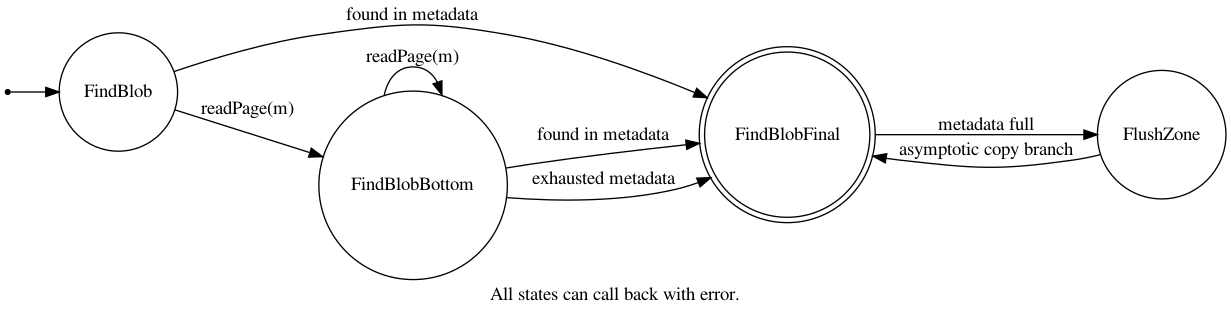
\includegraphics[width=1\linewidth]{FindBlob.png}
\captionof{figure}{\texttt{FindBlob} state machine}
\end{center}
\end{minipage}

\texttt{RemoveNamedBlob} and \texttt{ReplaceNamedBlob} are both extremely
simple once we have this model. They simply call \texttt{FindBlobFinal} with
\texttt{BLOB\_KILL} and \texttt{BLOB\_CREAT}, respectively. A new inode is
created with the name, pointing to its own data page as the previous page.
This inode will be found before any previous inodes of the same name. If
necessary, creating this inode will flush the active page to disk, possibly
provoking a block rescue. \texttt{ReplaceNamedBlob} invokes \texttt{ExtendBlob}
with the result. These are definitely the fastest ways to modify the blobstore,
as they waste no time absorbing the past.

\subsection{Reading and extending blobs}
Recall that the \texttt{blob\_t} returned by \texttt{OpenBlob} encodes the most
recent (i.e. last) inode (at the time of opening) from the blob. This is a
great place to be for appending, a great place for reading from small files
(since they are only one page), and a bad place for reading from the beginning
of large files.

\begin{minipage}{\textwidth}
\begin{center}
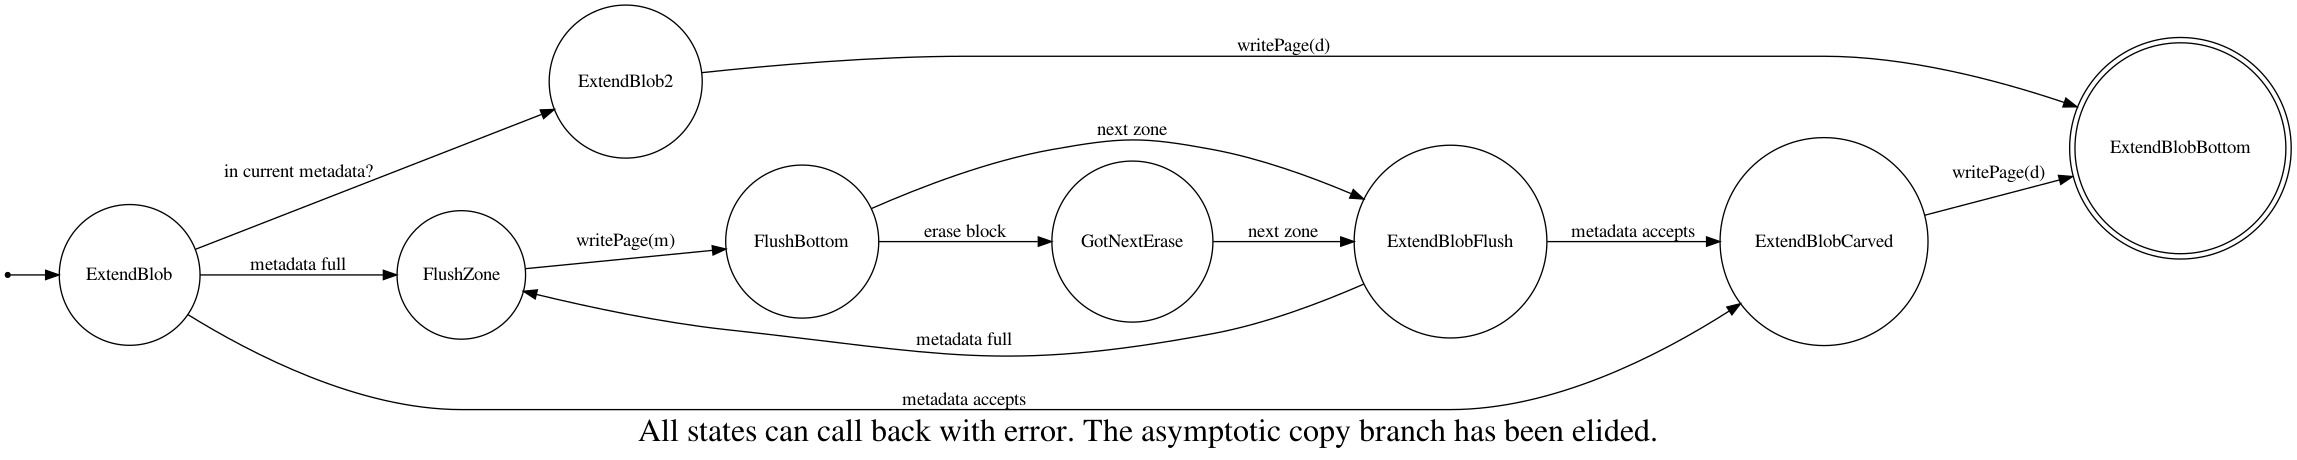
\includegraphics[width=1\linewidth]{ExtendBlob.png}
\captionof{figure}{\texttt{ExtendBlob} state machine}
\end{center}
\end{minipage}

The extension case is simple. We acquire a fresh inode from the
active page, and write its data page (locking in the inode) immediately. The
only exception is if our \texttt{blob\_t} is of the present epoch, in the
active zone, and its data page has not yet been written. In this case, no new
inode is necessary, and we write out the page. If a blob was created after this
one was created, but before this extension, that other blob will be ``locked in'' with an
empty first page. This wastes a page, which we'd like to recover in the next
epoch. For that reason, when we extend a blob using a reference to its locked-in
first page, the new inode is written as if it's the first inode of the blob---its
PrevPage field will specify itself.

For the read case, the metadata associated with the data
page (which might be the active metadata) is first read. From this metadata we
know the blob's length prior to this inode, and whether the page is a complete
(2KB) write (the length written to the Spare Area is 11 bits, and thus not
large enough to represent a full 2KB write. We keep the 12th necessary bit here
for an optimization, detailed momentarily. The length written to the Spare Area
is modulo $2^{11}$). We continue back through the metadata until reaching an
IncomingLen less than or equal to the requested offset. The referenced data
page is the earliest we need to read for the request.

We would need keep a list of page indices to ``come back through'', reading
data pages of the blob in order. This would require $\mathcal{O}(n)$ space on $n$ inodes.
For the worst case of a 2KB read made up of $2^{11}$ 1-byte writes, this
requires 4KB. Instead, we populate the read buffer in reverse. While moving
% CHECK THIS feels off-by-one %
backwards, we need data from any data page where the inode's IncomingLen plus
the data page's length is less than the read request's offset plus its own
length (so long as the IncomingLen + length is greater than or equal to the
read request's offset). We read up through the required data into the caller-provided
scratch buffer, and copy it into the request buffer. Not knowing the length
of the actual data page (we must read the Spare Area to know), we can't read
directly into the read buffer\footnote{Consider a 2KB read request
from offset 0 of a single-byte blob. This byte must go to the beginning of the buffer,
which is easily accomplished, but we must return 1 to the caller, not $2^{11}$.
In order to read the 1, we must read the entire page, which would blow out the
provided buffer. And thus we copy. Two distinct reads---one for the data, one for
the Spare Area---might or might not be faster than a large copy here.}.
If the Partial bit is \textit{not} set, however, we \textit{do} know the length
to be 2KB, and can do a zero-copy read. Since multipage files are strongly
encouraged to write full pages, this optimization can be significant for such
reads.

\begin{minipage}{\textwidth}
\begin{center}
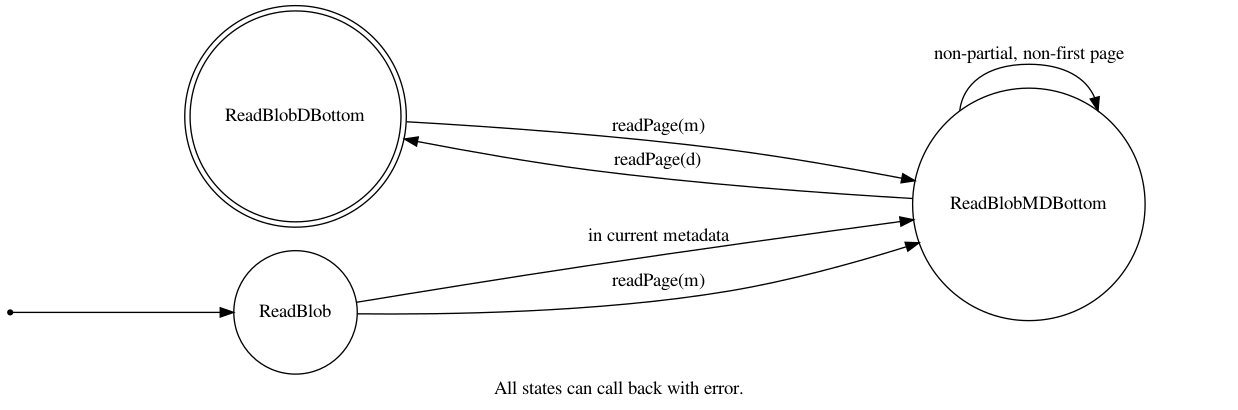
\includegraphics[width=.5\linewidth]{ReadBlob.png}
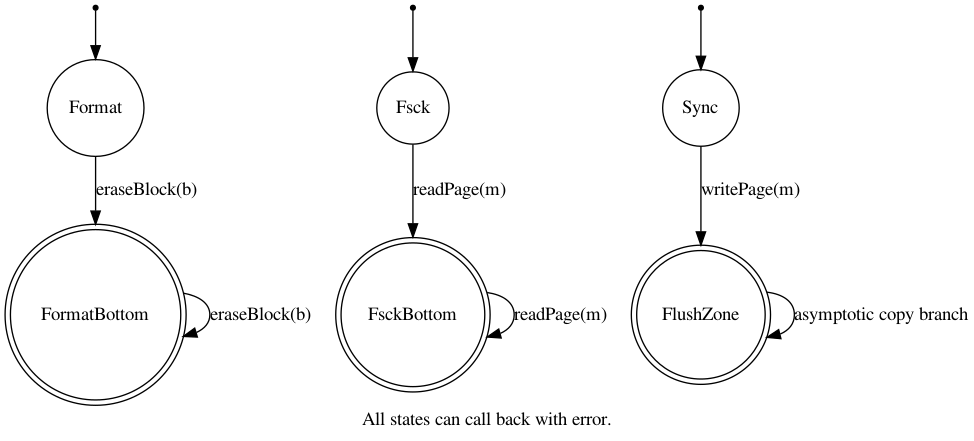
\includegraphics[width=.4\linewidth]{FSM.png}
\captionof{figure}{\texttt{ReadBlob}, \texttt{Format}, \texttt{Fsck}, and \texttt{Sync} state machines}
\end{center}
\end{minipage}

\subsection{Irregular operations}
\texttt{Format} erases each block in order. Its goal is to restore a NAND to
a fresh state.

\texttt{Fsck} reads each metadata page in order. Its goal is to verify that the
progression of nonces conforms to the rules outlined in Section \ref{callzones}.
There ought be zero, one, or two orderly processions downwards. One discontinuity
is allowed. The only other permitted progression is a series of uninitialized blocks
at the top of the NAND. It also ensures that all metadata pages can be read at
least once without ECC errors. It could obviously do more.

\texttt{Sync} flushes out metadata for the current block if any entries are
present, advancing the current zone to the first zone of the next block. This
is currently necessary to avoid data loss on shutdown, though I have ideas on
how to eliminate it.

\section{Future work} \label{futurework}
It is desirable to encode large files more efficiently. Currently, a file of
the maximum $2^{24}-1$ bytes requires 8192 inodes, and thus (in the best case)
530 pages of metadata, and attendant reads. When all of a zone is a single
blob, some different scheme ought be employed to encode this fact.
Unfortunately, it's unlikely that such a write could ever be performed as a
single ExtendBlob() operation, due to the RAM requirements of such a buffer.

It is not currently possible to use the two chips in parallel as a single,
unified blobstore. If placed on distinct SPI masters, they can be used in
parallel as two blobstores, or as a mirrored set. In any configuration---even
a single SPI master---they can be combined as a linear device. A unified
2Gbit namespace accessible at 2x32MHz, however, is not yet possible. Mirrored
sets could be implemented via superblocks for
maximum performance, requiring only a single SPI master. This would be especially
advantageous if the QSPI interface had been capable of driving the Winbonds.

An ECC failure reading a metadata page currently results in the blobstore being
brought offline. Given that ECC failures can often be recognized immediately
after programming, metapages should probably be read back following write,
remapped using the BBM LUTs, and written anew. In any case, a more graceful
recovery seems desirable.

We might be able to handle shutdown without a call to \texttt{Sync}, at least
for pages which actually wrote out data. The difficulty is twofold: we must
be able to recover the name for newly-created blobs (where would this be kept?),
and we must be able to absolutely distinguish written pages from random garbage.
This last requirement would be impossible, except that the user doesn't control
the Spare Area. By writing the epoch into the Spare Area, we can be pretty
well assured that we actually wrote the page.

There are surely forty thousand ways in which this design could be improved.

The implementation seems pretty solid, for whatever that's worth.

\section{Closing words}
A few weeks before receiving this contract, I (in a shameless rip-off of Douglas
Coupland's \textit{Microserfs}\parencite{microserfs}) remarked plaintively to
my wife, ``I'm 38. I've done everything you can do on a computer. Well, I've
never designed a filesystem.'' I appreciate the opportunity to correct that
deficiency.

I hope this writeup was informative! Hack on!\\

\textbf{\href{https://www.dsscaw.com/}{Dirty South Supercomputing}. Soak more cycles. Burn fewer dinosaurs.}
\vspace{1cm}

%%%%%%%%%%%%%%%%%%%%%%%%%%%%%%%%%%%%%%%%%%%%%%%%%%%%%%%%%%%%%%%%%%%%%%%%
\printbibliography
\vfill
\begin{minipage}{\textwidth}
\begin{center}

\includegraphics[width=.4\linewidth]{../dsscaw-purp-scaled.png}

\includegraphics[width=.5\linewidth]{south.png}
\end{center}
\end{minipage}
\end{document}
